%!TEX root = ../main.tex

\chapter{E2E simulation of 5G networks}
\label{chp:ns3}

\paragraph{}
As part of its contributions, this thesis introduces a preliminary end-to-end simulator for 5G \ac{NR} \ac{NTN} deployments. This simulator builds upon the ns3-mmwave simulation module, which accurately models the 5G \ac{NR} protocol stack, and has been recently extended with the 3GPP channel model for NTNs \cite{Sandri_2023}. This chapter describes this baseline, which has been used as the starting point for designing and developing an end-to-end simulator for 5G \ac{NR} \ac{NTN} deployments.

\section{Discrete events network simulators}
The network simulators scenario consists of two main categories: discrete events and real time simulators. The former option is the most performing one, since it allows for the processing of complex events even in less performing hardware. Real time simulators require more high-end hardware, otherwise the processing of complex events can slow down the whole simulation.

In discrete events simulators, each operation to be performed is associated to an event, and in turn, each event is associated with a set of instructions and its execution time. The simulation proceeds by processing and executing events, stepping from one to the next, as the simulation time passes. From the point of view of the simulation, each event is executed in zero time, since the time is stopped while executing a single event, and its course resumes only when transitioning between events scheduled at different times. If no events are scheduled to execute for a certain period of time, the simulation immediately transitions to the next scheduled one. This kind of behavior is what discerns discrete events simulators from their counterparts,  real-time simulators. As the simulation unfolds, events are sequentially executed, each of the former possibly scheduling new additional events. As an example, the event of a packet being transmitted in a network may generate the corresponding reception event after a set propagation delay \cite{review-ns3}.

The most popular simulation softwares are OMNeT++ \cite{omnetpp}, SWANS \cite{swans}, NetSim by TetCos \cite{netsim}, QualNet, ns-3, and its predecessor ns-2 \cite{ns3}. Their main characteristics are summarized in Table \ref{tab:simulators}, from \cite{review-ns3}, which posed the accent on the suitability of ns-3 for research purposes, highlighting its success amongst the scientific community.

\begin{table}[]
    \small
    \begin{tabular}{|c|lllll}
        \hline
            {\textbf{Tool}} &
            \multicolumn{1}{c|}{{\textbf{ns-3}}} &
            \multicolumn{1}{c|}{{\textbf{OMNET++}}} &
            \multicolumn{1}{c|}{{\textbf{SWANS}}} &
            \multicolumn{1}{c|}{{\textbf{NetSim}}} &
            \multicolumn{1}{c|}{{\textbf{QualNet}}}
            \\ \hline

            {Interface} &
            \begin{tabular}[c]{@{}l@{}}C++,\\ Python\end{tabular} &
            \begin{tabular}[c]{@{}l@{}}C++,\\ NED\end{tabular} &
            Java &
            \begin{tabular}[c]{@{}l@{}}C,\\ Java,\\ .NET\end{tabular} &
            Parsec
            \\ \hline

            {License} &
            Free &
            Academic &
            Free &
            Paid &
            Paid
            \\ \hline
            
            {Parallelism} &
            No &
            No &
            Yes &
            No &
            Yes
            \\ \hline

            {OS} &
            \begin{tabular}[c]{@{}l@{}}Linux,\\ FreeBSD,\\ MacOS\\ Windows\end{tabular} &
            \begin{tabular}[c]{@{}l@{}}Linux,\\ MacOS,\\ Windows\end{tabular} &
            \begin{tabular}[c]{@{}l@{}}Linux,\\ MacOS,\\ Windows\end{tabular} &
            Windows &
            \begin{tabular}[c]{@{}l@{}}Linux,\\ MacOS,\\ Windows,\\ Unix\end{tabular}
            \\ \hline

            {Mobility support} &
            Yes &
            No &
            Yes &
            Yes &
            Yes
            \\ \hline

            {GUI} &
            Limited &
            Yes &
            Yes &
            Yes &
            Yes
            \\ \hline
    \end{tabular}
    \caption{Network simulation software comparison \label{tab:simulators}}
\end{table}

\section{ns-3}
\label{sec:ns3_desc}

\begin{figure}[ht]
    \centering
    
\includegraphics[width=0.5\textwidth]{res/ns-3-notext.png}
    \caption{ns-3 logo \href{https://www.nsnam.org/}{nsnam.org}}
    \label{fig:ns3-logo}
\end{figure}

Being a modular, extensible, community-supported, full-stack network software simulation tool based on a discrete event approach, the ns-3 simulator was the software of choice to conduct the testing campaigns. It is an open source project licensed under the GNU GPLv2 license, thus allowing users to freely re-use the software and to introduce modifications to the codebase \cite{ns3-website}.

\paragraph{The community}
Being specifically targeted for the academic world, and for research, as well as being open-source, ns-3 sees a thriving community of developers and researchers, with an active forum\footnote{Link to google group about ns-3 \href{https://groups.google.com/g/ns-3-users}{groups.google.com/g/ns-3-users}}, a well maintained documentation and a lot of independent lectures, tutorials and articles. 

\paragraph{Modularity}
Ns-3 exhibits a modular philosophy. The base version provides the core of the simulator with a plethora of functionality, but lots of expansion modules have been coded by researchers and developers. The following sections present the ns3-ntn and ns3-mmwave modules, that were used in this thesis in order to provide an initial support to base our work on.


\section{Preliminary support for NTN NR simulations}
The ns3-mmwave module provides support for the simulation of 5G \ac{NR} stack, while \cite{Sandri_2023} provides a standard implementation of a non-terrestrial channel model, but the support for \ac{NR} stack in \ac{NTN} is still missing. These two modules are presented in this section, then further extended to obtain a ntn module capable of simulating the \ac{NR} stack in \ac{NTN}.

\subsection{Channel model}
The \ac{3GPP} channel modeling framework, described in TR 38.901 \cite{3gpp-tr-38.901}, which supports frequencies up to 100 GHz, statistically simulates both large and small scale fading parameters. Four different reference scenarios are specified: rural macto, urban macro, urban micro, and indoor hotspot. Furthermore, each scenario is subdivided in \ac{LOS} or N\ac{LOS} condition.

The remainder of this chapter briefly describes the \ac{3GPP} TR 38.901 channel model, with a focus on its extensions for modeling \ac{NTN} scenarios. For a comprehensive description of the baseline model, we instead refer the interested reader to \cite{channel-model-ns3}.

\subsubsection{Free space path loss}
The free space path loss is the major attenuation component in non-terrestrial links due to their length, and can be calculated as the ratio between the received power and the transmitted power with the well-known Friis formula 

\begin{equation}
    \frac{P_r}{P_t} = D_tD_r\left(\frac{\lambda}{4\pi d}\right)^2
    \label{eqn:fspl}
\end{equation}

Where $D_t$ and $D_r$ denote the directivities of the transmitting and receiving antennas, $\lambda$ is the wavelength and $d$ the distance.


\subsubsection{Atmospheric attenuation}
\paragraph{}
In addition to the free-space path loss that characterizes the majority of wireless communication systems, atmospheric absorption also plays an important role in attenuating certain frequency bands of the signal, as described in Figure \ref{fig:atmospheric-abs}. The peaks at 60 and 120 GHz are due to the resonance with molecular oxygen, while the peak at 180 GHz and the small hump at 25 GHz are due to the absorption from water vapor \cite{e-band-ammar}.

The nature of this phenomenon makes it susceptible to variations as the humidity rate varies, and different altitudes also lead to different absorption values.

\subsubsection{Shadowing}
Shadowing is a variation in the signal amplitude which stems from the latter reflection and scattering by surrounding objects, therefore arriving at the receiving antenna from many different paths. This causes multiple copies of the signal to be received, each copy having its own attenuation and phase, since the propagation paths and their distance are, in general, different. This effect can cause rapid fluctuations in the signal amplitude, due to either constructive or destructive interference.

\subsubsection{Additional factors}
Other factors causing additional attenuation are the presence of rain, cloudy conditions, the presence of fog, and different meteorological parameters. These factors are described in \cite{atm-effects-signal-prop}.

Furthermore, the different scenarios that the \ac{UE} can experience also have a major impact on its communication capabilities. Such scenarios are divided by \ac{3GPP} in four main categories: Dense urban, Urban, Suburban and Rural. In each scenario, the probability of having direct \ac{LOS} with a satellite differs, since the density of obstacles such as buildings varies depending on the situation.



\begin{figure}[ht]
    \centering
    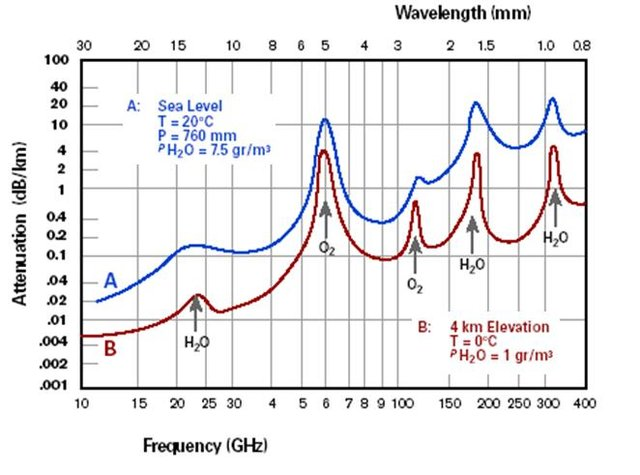
\includegraphics[width=0.8\textwidth]{res/atm-absorp.jpg}
    \caption{Atmospheric absorption in dB/km, from \cite{e-band-ammar}}
    \label{fig:atmospheric-abs}
\end{figure}


\subsection{NS-3 channel model implementation}

\paragraph{}
A ns-3 module to simulate a non-terrestrial channel model has already been implemented, and is available open-source\footnote{\href{https://gitlab.com/mattiasandri/ns-3-ntn/-/tree/ntn-dev?ref_type=heads}{gitlab.com/mattiasandri}}. This model is based on the \ac{3GPP} specifications as detailed in the standard TR 38.811 \cite{3gpp-tr-38.811}, paving the way for simulating wireless channels in space.

The implementation of such channel model required the modification and the creation of some ns-3 classes. This work is extensively described in \cite{Sandri_2023}, while a brief overview is hereby reported.

\subsubsection{Modified classes}
\begin{itemize}
    \item \texttt{ThreeGppChannelModel}: different parameters were introduced in order for this class to be able to correctly characterize the non-terrestrial use case. The large number of \ac{NTN}-related parameters made necessary the use of data structures such as maps to store them, and the mobility model of both the satellite and the \ac{UE} have been integrated in the computation of the small scale parameters returned by the class.
    \item \texttt{GeographicPositions}: class tasked with the various conversions between different coordinates systems such as longitude, latitude and altitude, the Geocentric Cartesian system (also called Earth Centric Earth Fixed or ECEF), and the local tangent plane coordinate system expressing the position in North, East and Up coordinates \cite{wiki_coords}. All those three systems are depicted in Fig. \ref{fig:coord-syst}.
\end{itemize}
\subsubsection{New classes}
\begin{itemize}
    \item \texttt{ThreeGppNTNScenarioChannelConditionModel}: the main task of this class is to store the channel state and condition. Four new classes were developed to store the four possible scenarios described by \ac{3GPP}:
    \begin{itemize}
        \item Dense urban,
        \item Urban,
        \item Suburban,
        \item Rural
    \end{itemize}
    \item \texttt{ThreeGppNTNScenarioPropagationLossModel}: four different scenarios are implemented in as many classes. Such classes are tasked with the computation of the total path loss, which includes contributions from the standard free space path loss, atmospheric absorption, scintillation, fading and clutter loss.
    \item \texttt{GeocentricConstantPositionMobilityModel}: allows for the use of terrestrial coordinates to position \ac{UE}s on the Earth surface. Conversions amongst different systems are done using the \texttt{GeographicPositions} class described above.
    \item \texttt{CircularApertureAntennaModel}: an exact implementation of the parabolic antenna model, making use of a new and efficient C++ function for the computation of Bessel functions required when considering the radiation pattern of aperture antennas \cite{rad-patterns}. Differently from the default ns-3 implementation, this newer version does not introduce approximations.
\end{itemize}




\begin{figure}[ht]
    \centering
    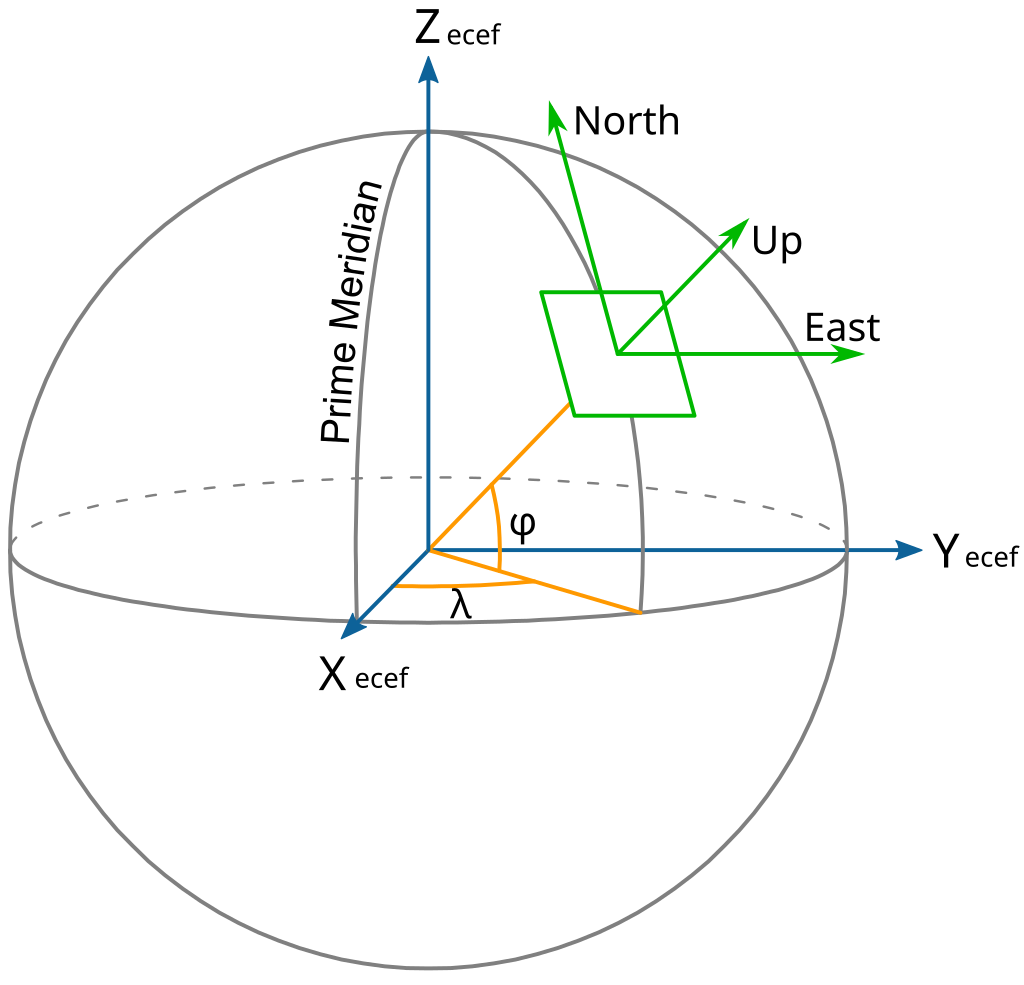
\includegraphics[width=0.5\textwidth]{res/coord_systems.png}
    \caption{Showcase of different coordinates systems \cite{wiki_coords}}
    \label{fig:coord-syst}
\end{figure}


\section{mmWave module}

The Ns-3-mmWave module, created by the NYU Wireless Research Centre and the SIGNET Research Group at University of Padova, enables the end-to-end simulation of standard-compliant 5G \ac{NR} cellular networks. \ac{3GPP}-specified statistical channel models are implemented, with modular and highly customisable classes \cite{e2e-sim-mmwave}.

After an initial study of the mmWave module, its implementation in a non-terrestrial scenario was devised, and numerous modifications were implemented to its classes in order to overcome all the problems that initially caused it to malfunction. These modifications are detailed in the following chapters, and represent an importnat original contribution of this thesis that was not previously treated by the literature. 

In particular, we modified the classes of the radio stacks of both the base station and \ac{UE} (\texttt{MmWaveEnbNetDevice} and \texttt{MmWaveUeNetDevice}), as well as the classes implementing the MAC layer and scheduler, namely \texttt{MmWaveEnbMac}, \texttt{MmWaveUeMac}, and \texttt{MmWaveMacScheduler}.

\section{Use in this work}
\paragraph{}
The ns3-mmWave module enables the simulation of the 5G \ac{NR} protocol stack, while the ns3-ntn module \cite{Sandri_2023} provides a \ac{3GPP}-like channel model for \ac{NTN}s. However, prior to the work done in this thesis, the simulation of a joint scenario of \ac{NR} stack in a non-terrestrial scenario was not possible, since the network stack was not designed to accomodate for the propagation delays exhibited by \ac{NTN} links.
The two modules were not able to operate in conjunction. Our work made non-terrestrial \ac{NR} simulation possible.



